\documentclass[a4paper]{book}
\usepackage{a4wide}
\usepackage{makeidx}
\usepackage{graphicx}
\usepackage{multicol}
\usepackage{float}
\usepackage{listings}
\usepackage{color}
\usepackage{textcomp}
\usepackage{alltt}
\usepackage[utf8]{inputenc}
\usepackage[brazil]{babel}
\usepackage{doxygen}
\lstset{language=C++,inputencoding=utf8,basicstyle=\footnotesize,breaklines=true,breakatwhitespace=true,tabsize=8,numbers=left }
\makeindex
\setcounter{tocdepth}{3}
\renewcommand{\footrulewidth}{0.4pt}
\begin{document}
\begin{titlepage}
\vspace*{7cm}
\begin{center}
{\Large Ginga-\/CC P2P }\\
\vspace*{1cm}
{\large Gerado por Doxygen 1.6.3}\\
\vspace*{0.5cm}
{\small Wed Nov 17 16:35:47 2010}\\
\end{center}
\end{titlepage}
\clearemptydoublepage
\pagenumbering{roman}
\tableofcontents
\clearemptydoublepage
\pagenumbering{arabic}
\chapter{Índice dos Componentes}
\section{Hierarquia de Classes}
Esta lista de hierarquias está parcialmente ordenada (ordem alfabética):\begin{DoxyCompactList}
\item \contentsline{section}{br::usp::icmc::intermidia::ginga::core::p2p::ChatTask}{\pageref{classbr_1_1usp_1_1icmc_1_1intermidia_1_1ginga_1_1core_1_1p2p_1_1ChatTask}}{}
\item \contentsline{section}{br::usp::icmc::intermidia::ginga::core::p2p::FileShareClient}{\pageref{classbr_1_1usp_1_1icmc_1_1intermidia_1_1ginga_1_1core_1_1p2p_1_1FileShareClient}}{}
\item \contentsline{section}{br::usp::icmc::intermidia::ginga::core::p2p::IP2PEventListener}{\pageref{classbr_1_1usp_1_1icmc_1_1intermidia_1_1ginga_1_1core_1_1p2p_1_1IP2PEventListener}}{}
\item \contentsline{section}{br::usp::icmc::intermidia::ginga::core::p2p::IP2PManager}{\pageref{classbr_1_1usp_1_1icmc_1_1intermidia_1_1ginga_1_1core_1_1p2p_1_1IP2PManager}}{}
\begin{DoxyCompactList}
\item \contentsline{section}{br::usp::icmc::intermidia::ginga::core::p2p::P2PManager}{\pageref{classbr_1_1usp_1_1icmc_1_1intermidia_1_1ginga_1_1core_1_1p2p_1_1P2PManager}}{}
\end{DoxyCompactList}
\end{DoxyCompactList}

\chapter{Índice dos Componentes}
\section{Lista de Componentes}
Aqui estão as classes, estruturas, uniões e interfaces e suas respectivas descrições:\begin{DoxyCompactList}
\item\contentsline{section}{{\bf br::usp::icmc::intermidia::ginga::p2ptest::GraphicInterface} }{\pageref{classbr_1_1usp_1_1icmc_1_1intermidia_1_1ginga_1_1p2ptest_1_1GraphicInterface}}{}
\item\contentsline{section}{{\bf br::usp::icmc::intermidia::ginga::p2ptest::GraphicList} }{\pageref{classbr_1_1usp_1_1icmc_1_1intermidia_1_1ginga_1_1p2ptest_1_1GraphicList}}{}
\item\contentsline{section}{{\bf br::usp::icmc::intermidia::ginga::p2ptest::P2PTest} }{\pageref{classbr_1_1usp_1_1icmc_1_1intermidia_1_1ginga_1_1p2ptest_1_1P2PTest}}{}
\end{DoxyCompactList}

\chapter{Índice dos Arquivos}
\section{Lista de Arquivos}
Esta é a lista de todos os arquivos documentados e suas respectivas descrições:\begin{DoxyCompactList}
\item\contentsline{section}{include/{\bf ChatTask.h} }{\pageref{ChatTask_8h}}{}
\item\contentsline{section}{include/{\bf FileShareClient.h} }{\pageref{FileShareClient_8h}}{}
\item\contentsline{section}{include/{\bf IP2PEventListener.h} }{\pageref{IP2PEventListener_8h}}{}
\item\contentsline{section}{include/{\bf IP2PManager.h} }{\pageref{IP2PManager_8h}}{}
\item\contentsline{section}{include/{\bf P2PManager.h} }{\pageref{P2PManager_8h}}{}
\item\contentsline{section}{src/{\bf FileShareClient.cpp} }{\pageref{FileShareClient_8cpp}}{}
\item\contentsline{section}{src/{\bf P2PManager.cpp} }{\pageref{P2PManager_8cpp}}{}
\end{DoxyCompactList}

\chapter{Classes}
\section{Referência da Classe br::usp::icmc::intermidia::ginga::core::p2p::ChatTask}
\label{classbr_1_1usp_1_1icmc_1_1intermidia_1_1ginga_1_1core_1_1p2p_1_1ChatTask}\index{br::usp::icmc::intermidia::ginga::core::p2p::ChatTask@{br::usp::icmc::intermidia::ginga::core::p2p::ChatTask}}


{\ttfamily \#include $<$ChatTask.h$>$}

\subsection*{Métodos Públicos}
\begin{DoxyCompactItemize}
\item 
{\bf ChatTask} (talk\_\-base::Task $\ast$parent)
\item 
virtual {\bf $\sim$ChatTask} ()
\item 
void {\bf sendChatMessage} (buzz::Jid $\ast$sendToJid, const string \&text)
\end{DoxyCompactItemize}
\subsection*{Atributos Públicos}
\begin{DoxyCompactItemize}
\item 
sigslot::signal2$<$ buzz::Jid, const string \& $>$ {\bf SignalIncomingChat}
\end{DoxyCompactItemize}
\subsection*{Métodos Protegidos}
\begin{DoxyCompactItemize}
\item 
virtual int {\bfseries ProcessStart} ()\label{classbr_1_1usp_1_1icmc_1_1intermidia_1_1ginga_1_1core_1_1p2p_1_1ChatTask_a0c62b48a707d1f844e9c50f5e8865a58}

\item 
virtual bool {\bfseries HandleStanza} (const buzz::XmlElement $\ast$stanza)\label{classbr_1_1usp_1_1icmc_1_1intermidia_1_1ginga_1_1core_1_1p2p_1_1ChatTask_ae3fcb7b611b6cc69ec0852bbc593381a}

\end{DoxyCompactItemize}
\subsection*{Atributos Protegidos}
\begin{DoxyCompactItemize}
\item 
HLoggerPtr {\bf logger}\label{classbr_1_1usp_1_1icmc_1_1intermidia_1_1ginga_1_1core_1_1p2p_1_1ChatTask_a05fc7c4045c19a95b582fa4d5b82c011}

\begin{DoxyCompactList}\small\item\em Componente auxiliar para realização de logs. \item\end{DoxyCompactList}\end{DoxyCompactItemize}


\subsection{Descrição Detalhada}
Esta classe foi inspirada na classe de mesmo nome do projeto gtalX ({\tt http://sites.google.com/site/jozsefbekes/Home/gtalx})

Tem como finalidade permitir o envio e recebimento de mensagens de texto. 

\subsection{Construtores \& Destrutores}
\index{br::usp::icmc::intermidia::ginga::core::p2p::ChatTask@{br::usp::icmc::intermidia::ginga::core::p2p::ChatTask}!ChatTask@{ChatTask}}
\index{ChatTask@{ChatTask}!br::usp::icmc::intermidia::ginga::core::p2p::ChatTask@{br::usp::icmc::intermidia::ginga::core::p2p::ChatTask}}
\subsubsection[{ChatTask}]{\setlength{\rightskip}{0pt plus 5cm}br::usp::icmc::intermidia::ginga::core::p2p::ChatTask::ChatTask (talk\_\-base::Task $\ast$ {\em parent})}\label{classbr_1_1usp_1_1icmc_1_1intermidia_1_1ginga_1_1core_1_1p2p_1_1ChatTask_abcf6614965be5ae7204d4f57c09fdb05}
Construtor da Task responsável pelo chat.


\begin{DoxyParams}{Parâmetros}
\item[{\em parent}]Task pai. \end{DoxyParams}


Referências logger.

\index{br::usp::icmc::intermidia::ginga::core::p2p::ChatTask@{br::usp::icmc::intermidia::ginga::core::p2p::ChatTask}!$\sim$ChatTask@{$\sim$ChatTask}}
\index{$\sim$ChatTask@{$\sim$ChatTask}!br::usp::icmc::intermidia::ginga::core::p2p::ChatTask@{br::usp::icmc::intermidia::ginga::core::p2p::ChatTask}}
\subsubsection[{$\sim$ChatTask}]{\setlength{\rightskip}{0pt plus 5cm}br::usp::icmc::intermidia::ginga::core::p2p::ChatTask::$\sim$ChatTask ()\hspace{0.3cm}{\ttfamily  [virtual]}}\label{classbr_1_1usp_1_1icmc_1_1intermidia_1_1ginga_1_1core_1_1p2p_1_1ChatTask_a142f2a4487d0e8cd87873f1837bc996c}
Destrutor da Task responsável pelo chat. 

Referências logger.



\subsection{Métodos}
\index{br::usp::icmc::intermidia::ginga::core::p2p::ChatTask@{br::usp::icmc::intermidia::ginga::core::p2p::ChatTask}!sendChatMessage@{sendChatMessage}}
\index{sendChatMessage@{sendChatMessage}!br::usp::icmc::intermidia::ginga::core::p2p::ChatTask@{br::usp::icmc::intermidia::ginga::core::p2p::ChatTask}}
\subsubsection[{sendChatMessage}]{\setlength{\rightskip}{0pt plus 5cm}void br::usp::icmc::intermidia::ginga::core::p2p::ChatTask::sendChatMessage (buzz::Jid $\ast$ {\em sendToJid}, \/  const string \& {\em text})}\label{classbr_1_1usp_1_1icmc_1_1intermidia_1_1ginga_1_1core_1_1p2p_1_1ChatTask_a08f15eb0a25da642c5444ebff761e190}
Envia uma mensagem de texto para um determinado amigo.


\begin{DoxyParams}{Parâmetros}
\item[{\em sendToJid}]Amigo que irá receber a mensagem \item[{\em text}]Mensagem a ser enviada \end{DoxyParams}


Referências logger.



\subsection{Atributos}
\index{br::usp::icmc::intermidia::ginga::core::p2p::ChatTask@{br::usp::icmc::intermidia::ginga::core::p2p::ChatTask}!SignalIncomingChat@{SignalIncomingChat}}
\index{SignalIncomingChat@{SignalIncomingChat}!br::usp::icmc::intermidia::ginga::core::p2p::ChatTask@{br::usp::icmc::intermidia::ginga::core::p2p::ChatTask}}
\subsubsection[{SignalIncomingChat}]{\setlength{\rightskip}{0pt plus 5cm}sigslot::signal2$<$buzz::Jid , const string\& $>$ {\bf br::usp::icmc::intermidia::ginga::core::p2p::ChatTask::SignalIncomingChat}}\label{classbr_1_1usp_1_1icmc_1_1intermidia_1_1ginga_1_1core_1_1p2p_1_1ChatTask_aadea820b55f7ff1ed5a75ea416369c30}
Slot pelo qual serão notificadas ocorrências de recebimento mensagens de texto. 

A documentação para esta classe foi gerada a partir dos seguintes arquivos:\begin{DoxyCompactItemize}
\item 
include/{\bf ChatTask.h}\item 
src/ChatTask.cpp\end{DoxyCompactItemize}

\section{Referência da Classe br::usp::icmc::intermidia::ginga::core::p2p::FileShareClient}
\label{classbr_1_1usp_1_1icmc_1_1intermidia_1_1ginga_1_1core_1_1p2p_1_1FileShareClient}\index{br::usp::icmc::intermidia::ginga::core::p2p::FileShareClient@{br::usp::icmc::intermidia::ginga::core::p2p::FileShareClient}}


{\ttfamily \#include $<$FileShareClient.h$>$}

\subsection*{Tipos Públicos}
\begin{DoxyCompactItemize}
\item 
enum {\bf State} \{ \par
{\bf OFFER} =  0, 
{\bf TRANSFER} =  1, 
{\bf COMPLETE} =  2, 
{\bf LOCAL\_\-CANCEL} =  3, 
\par
{\bf REMOTE\_\-CANCEL} =  4, 
{\bf FAILURE} =  5
 \}
\item 
enum \{ {\bfseries MSG\_\-STOP}, 
{\bfseries MSG\_\-DECLINE}, 
{\bfseries MSG\_\-ACCEPT}
 \}
\end{DoxyCompactItemize}
\subsection*{Métodos Públicos}
\begin{DoxyCompactItemize}
\item 
{\bf FileShareClient} (std::string root\_\-dir)
\item 
{\bf $\sim$FileShareClient} ()
\item 
void {\bf setListener} ({\bf IP2PEventListener} $\ast$listener)
\item 
void {\bf setStatus} (buzz::Status::Show show, string message)
\item 
void {\bf sendFiles} (vector$<$ string $>$ $\ast$files, const buzz::Jid \&send\_\-to, map$<$ string, buzz::Status $>$ $\ast$roster)
\item 
void {\bf onSignon} (cricket::SessionManager $\ast$session\_\-manager, const buzz::Jid jid)
\item 
void {\bf onPossibleDestinationOnline} (const buzz::Status \&status)
\end{DoxyCompactItemize}


\subsection{Descrição Detalhada}
Classe responsável pela troca de arquivos entre clientes XMPP. 

\subsection{Enumerações}
\subsubsection[{"@0}]{\setlength{\rightskip}{0pt plus 5cm}anonymous enum}\label{classbr_1_1usp_1_1icmc_1_1intermidia_1_1ginga_1_1core_1_1p2p_1_1FileShareClient_a4e681ca7516e609028da94b3476ca412}
Possíveis valores para mensagens a serem trocadas entre threads através da MessageQueue. \index{br::usp::icmc::intermidia::ginga::core::p2p::FileShareClient@{br::usp::icmc::intermidia::ginga::core::p2p::FileShareClient}!State@{State}}
\index{State@{State}!br::usp::icmc::intermidia::ginga::core::p2p::FileShareClient@{br::usp::icmc::intermidia::ginga::core::p2p::FileShareClient}}
\subsubsection[{State}]{\setlength{\rightskip}{0pt plus 5cm}enum {\bf br::usp::icmc::intermidia::ginga::core::p2p::FileShareClient::State}}\label{classbr_1_1usp_1_1icmc_1_1intermidia_1_1ginga_1_1core_1_1p2p_1_1FileShareClient_a8107d8473b5b423f212ffa238e230894}
\begin{Desc}
\item[Valores enumerados: ]\par
\begin{description}
\index{OFFER@{OFFER}!br::usp::icmc::intermidia::ginga::core::p2p::FileShareClient@{br::usp::icmc::intermidia::ginga::core::p2p::FileShareClient}}\index{br::usp::icmc::intermidia::ginga::core::p2p::FileShareClient@{br::usp::icmc::intermidia::ginga::core::p2p::FileShareClient}!OFFER@{OFFER}}\item[{\em 
OFFER\label{classbr_1_1usp_1_1icmc_1_1intermidia_1_1ginga_1_1core_1_1p2p_1_1FileShareClient_a8107d8473b5b423f212ffa238e230894add74e92b9f133b492dba78c528f10161}
}]Alguem está lhe oferecendo arquivos (acompanha um manifesto). \index{TRANSFER@{TRANSFER}!br::usp::icmc::intermidia::ginga::core::p2p::FileShareClient@{br::usp::icmc::intermidia::ginga::core::p2p::FileShareClient}}\index{br::usp::icmc::intermidia::ginga::core::p2p::FileShareClient@{br::usp::icmc::intermidia::ginga::core::p2p::FileShareClient}!TRANSFER@{TRANSFER}}\item[{\em 
TRANSFER\label{classbr_1_1usp_1_1icmc_1_1intermidia_1_1ginga_1_1core_1_1p2p_1_1FileShareClient_a8107d8473b5b423f212ffa238e230894a9523203e14bfb4cc1ea7bb403d05f59d}
}]Tranferência iniciada. \index{COMPLETE@{COMPLETE}!br::usp::icmc::intermidia::ginga::core::p2p::FileShareClient@{br::usp::icmc::intermidia::ginga::core::p2p::FileShareClient}}\index{br::usp::icmc::intermidia::ginga::core::p2p::FileShareClient@{br::usp::icmc::intermidia::ginga::core::p2p::FileShareClient}!COMPLETE@{COMPLETE}}\item[{\em 
COMPLETE\label{classbr_1_1usp_1_1icmc_1_1intermidia_1_1ginga_1_1core_1_1p2p_1_1FileShareClient_a8107d8473b5b423f212ffa238e230894a5b6aeb6180356da800dd5d8cac896114}
}]Transferência completada. \index{LOCAL\_\-CANCEL@{LOCAL\_\-CANCEL}!br::usp::icmc::intermidia::ginga::core::p2p::FileShareClient@{br::usp::icmc::intermidia::ginga::core::p2p::FileShareClient}}\index{br::usp::icmc::intermidia::ginga::core::p2p::FileShareClient@{br::usp::icmc::intermidia::ginga::core::p2p::FileShareClient}!LOCAL\_\-CANCEL@{LOCAL\_\-CANCEL}}\item[{\em 
LOCAL\_\-CANCEL\label{classbr_1_1usp_1_1icmc_1_1intermidia_1_1ginga_1_1core_1_1p2p_1_1FileShareClient_a8107d8473b5b423f212ffa238e230894ac7920ab10b5d25799da57c7d391f8bfc}
}]Transferência cancelada localmente. \index{REMOTE\_\-CANCEL@{REMOTE\_\-CANCEL}!br::usp::icmc::intermidia::ginga::core::p2p::FileShareClient@{br::usp::icmc::intermidia::ginga::core::p2p::FileShareClient}}\index{br::usp::icmc::intermidia::ginga::core::p2p::FileShareClient@{br::usp::icmc::intermidia::ginga::core::p2p::FileShareClient}!REMOTE\_\-CANCEL@{REMOTE\_\-CANCEL}}\item[{\em 
REMOTE\_\-CANCEL\label{classbr_1_1usp_1_1icmc_1_1intermidia_1_1ginga_1_1core_1_1p2p_1_1FileShareClient_a8107d8473b5b423f212ffa238e230894a083d96a14e3d98e812e2cd3f5308d165}
}]Transferência cancelada remotamente. \index{FAILURE@{FAILURE}!br::usp::icmc::intermidia::ginga::core::p2p::FileShareClient@{br::usp::icmc::intermidia::ginga::core::p2p::FileShareClient}}\index{br::usp::icmc::intermidia::ginga::core::p2p::FileShareClient@{br::usp::icmc::intermidia::ginga::core::p2p::FileShareClient}!FAILURE@{FAILURE}}\item[{\em 
FAILURE\label{classbr_1_1usp_1_1icmc_1_1intermidia_1_1ginga_1_1core_1_1p2p_1_1FileShareClient_a8107d8473b5b423f212ffa238e230894a78d4266954c1a008e7859d21faff3314}
}]Falha durante transferência. \end{description}
\end{Desc}



\subsection{Construtores \& Destrutores}
\index{br::usp::icmc::intermidia::ginga::core::p2p::FileShareClient@{br::usp::icmc::intermidia::ginga::core::p2p::FileShareClient}!FileShareClient@{FileShareClient}}
\index{FileShareClient@{FileShareClient}!br::usp::icmc::intermidia::ginga::core::p2p::FileShareClient@{br::usp::icmc::intermidia::ginga::core::p2p::FileShareClient}}
\subsubsection[{FileShareClient}]{\setlength{\rightskip}{0pt plus 5cm}br::usp::icmc::intermidia::ginga::core::p2p::FileShareClient::FileShareClient (std::string {\em root\_\-dir})}\label{classbr_1_1usp_1_1icmc_1_1intermidia_1_1ginga_1_1core_1_1p2p_1_1FileShareClient_a91d30e909ab8c51c53d1451d4b7dfcef}
Constrói um objeto \doxyref{FileShareClient}{pag.}{classbr_1_1usp_1_1icmc_1_1intermidia_1_1ginga_1_1core_1_1p2p_1_1FileShareClient} já passando tudo que é necessário para realizar uma conexão.


\begin{DoxyParams}{Parâmetros}
\item[{\em root\_\-dir}]Diretório onde os arquivos serão procurados ou escritos. \end{DoxyParams}
\index{br::usp::icmc::intermidia::ginga::core::p2p::FileShareClient@{br::usp::icmc::intermidia::ginga::core::p2p::FileShareClient}!$\sim$FileShareClient@{$\sim$FileShareClient}}
\index{$\sim$FileShareClient@{$\sim$FileShareClient}!br::usp::icmc::intermidia::ginga::core::p2p::FileShareClient@{br::usp::icmc::intermidia::ginga::core::p2p::FileShareClient}}
\subsubsection[{$\sim$FileShareClient}]{\setlength{\rightskip}{0pt plus 5cm}br::usp::icmc::intermidia::ginga::core::p2p::FileShareClient::$\sim$FileShareClient ()}\label{classbr_1_1usp_1_1icmc_1_1intermidia_1_1ginga_1_1core_1_1p2p_1_1FileShareClient_a92af93ef3499961dbe6b6e45ac6b0b5c}
Destrói um objeto \doxyref{FileShareClient}{pag.}{classbr_1_1usp_1_1icmc_1_1intermidia_1_1ginga_1_1core_1_1p2p_1_1FileShareClient}. 

\subsection{Métodos}
\index{br::usp::icmc::intermidia::ginga::core::p2p::FileShareClient@{br::usp::icmc::intermidia::ginga::core::p2p::FileShareClient}!onPossibleDestinationOnline@{onPossibleDestinationOnline}}
\index{onPossibleDestinationOnline@{onPossibleDestinationOnline}!br::usp::icmc::intermidia::ginga::core::p2p::FileShareClient@{br::usp::icmc::intermidia::ginga::core::p2p::FileShareClient}}
\subsubsection[{onPossibleDestinationOnline}]{\setlength{\rightskip}{0pt plus 5cm}void br::usp::icmc::intermidia::ginga::core::p2p::FileShareClient::onPossibleDestinationOnline (const buzz::Status \& {\em status})}\label{classbr_1_1usp_1_1icmc_1_1intermidia_1_1ginga_1_1core_1_1p2p_1_1FileShareClient_aa216e2d67c19e22c6bd3a71315019bb9}
Método chamado quando algum usuário fica online, para que esta classe possa checar se existe algum item que está pendente para ser enviado para esse usuário.


\begin{DoxyParams}{Parâmetros}
\item[{\em status}]Informações sobre o usuário que ficou online. \end{DoxyParams}
\index{br::usp::icmc::intermidia::ginga::core::p2p::FileShareClient@{br::usp::icmc::intermidia::ginga::core::p2p::FileShareClient}!onSignon@{onSignon}}
\index{onSignon@{onSignon}!br::usp::icmc::intermidia::ginga::core::p2p::FileShareClient@{br::usp::icmc::intermidia::ginga::core::p2p::FileShareClient}}
\subsubsection[{onSignon}]{\setlength{\rightskip}{0pt plus 5cm}void br::usp::icmc::intermidia::ginga::core::p2p::FileShareClient::onSignon (cricket::SessionManager $\ast$ {\em session\_\-manager}, \/  const buzz::Jid {\em jid})}\label{classbr_1_1usp_1_1icmc_1_1intermidia_1_1ginga_1_1core_1_1p2p_1_1FileShareClient_acc096dd9ed0f906d22a3b168da216be2}
Método chamado depois que uma conexão é estabelecida. Envia informação de presença e se registra para receber notificações de presença de outros.


\begin{DoxyParams}{Parâmetros}
\item[{\em session\_\-manager}]O gerenciador da sessão atual. \item[{\em jid}]O endereço XMPP do usuário. \end{DoxyParams}
\index{br::usp::icmc::intermidia::ginga::core::p2p::FileShareClient@{br::usp::icmc::intermidia::ginga::core::p2p::FileShareClient}!sendFiles@{sendFiles}}
\index{sendFiles@{sendFiles}!br::usp::icmc::intermidia::ginga::core::p2p::FileShareClient@{br::usp::icmc::intermidia::ginga::core::p2p::FileShareClient}}
\subsubsection[{sendFiles}]{\setlength{\rightskip}{0pt plus 5cm}void br::usp::icmc::intermidia::ginga::core::p2p::FileShareClient::sendFiles (vector$<$ string $>$ $\ast$ {\em files}, \/  const buzz::Jid \& {\em send\_\-to}, \/  map$<$ string, buzz::Status $>$ $\ast$ {\em roster})}\label{classbr_1_1usp_1_1icmc_1_1intermidia_1_1ginga_1_1core_1_1p2p_1_1FileShareClient_ae880077dd0b559a98eeb83fda410b7b2}
Envia arquivos e diretórios para um determinado amigo.


\begin{DoxyParams}{Parâmetros}
\item[{\em files}]Vetor contendo os caminhos dos arquivos e diretórios que serão enviados \item[{\em jid}]Identificador o amigo que irá receber os arquivos \end{DoxyParams}
\index{br::usp::icmc::intermidia::ginga::core::p2p::FileShareClient@{br::usp::icmc::intermidia::ginga::core::p2p::FileShareClient}!setListener@{setListener}}
\index{setListener@{setListener}!br::usp::icmc::intermidia::ginga::core::p2p::FileShareClient@{br::usp::icmc::intermidia::ginga::core::p2p::FileShareClient}}
\subsubsection[{setListener}]{\setlength{\rightskip}{0pt plus 5cm}void br::usp::icmc::intermidia::ginga::core::p2p::FileShareClient::setListener ({\bf IP2PEventListener} $\ast$ {\em listener})}\label{classbr_1_1usp_1_1icmc_1_1intermidia_1_1ginga_1_1core_1_1p2p_1_1FileShareClient_a89bea2344d930cfc0e0149630136e18d}
Permite setar o objeto responsável por tratar mudanças de estado relacionadas a trasnferência de arquivos e pastas, inclusive o recebimento de oferecimento de um item.


\begin{DoxyParams}{Parâmetros}
\item[{\em listener}]Observador que será notificado quando ocorrer qualquer mudança de estado relacionada a transferência de algum arquivo. \end{DoxyParams}
\index{br::usp::icmc::intermidia::ginga::core::p2p::FileShareClient@{br::usp::icmc::intermidia::ginga::core::p2p::FileShareClient}!setStatus@{setStatus}}
\index{setStatus@{setStatus}!br::usp::icmc::intermidia::ginga::core::p2p::FileShareClient@{br::usp::icmc::intermidia::ginga::core::p2p::FileShareClient}}
\subsubsection[{setStatus}]{\setlength{\rightskip}{0pt plus 5cm}void br::usp::icmc::intermidia::ginga::core::p2p::FileShareClient::setStatus (buzz::Status::Show {\em show}, \/  string {\em message})}\label{classbr_1_1usp_1_1icmc_1_1intermidia_1_1ginga_1_1core_1_1p2p_1_1FileShareClient_a7cca6557f5606ee125481b317c6a70d3}
Permite definir o próprio status.


\begin{DoxyParams}{Parâmetros}
\item[{\em show}]Status a ser utilizado. \item[{\em message}]Mensagem personalizada opcional. \end{DoxyParams}


A documentação para esta classe foi gerada a partir dos seguintes arquivos:\begin{DoxyCompactItemize}
\item 
include/{\bf FileShareClient.h}\item 
src/{\bf FileShareClient.cpp}\end{DoxyCompactItemize}

\section{Referência da Classe br::usp::icmc::intermidia::ginga::core::p2p::IP2PEventListener}
\label{classbr_1_1usp_1_1icmc_1_1intermidia_1_1ginga_1_1core_1_1p2p_1_1IP2PEventListener}\index{br::usp::icmc::intermidia::ginga::core::p2p::IP2PEventListener@{br::usp::icmc::intermidia::ginga::core::p2p::IP2PEventListener}}


{\ttfamily \#include $<$IP2PEventListener.h$>$}

\subsection*{Métodos Públicos}
\begin{DoxyCompactItemize}
\item 
virtual {\bf $\sim$IP2PEventListener} ()
\item 
virtual void {\bf transferStateChanged} ({\bf FileShareClient::State} state, const cricket::FileShareManifest $\ast$manifest)=0
\item 
virtual void {\bf stateChanged} (buzz::XmppEngine::State state)=0
\item 
virtual void {\bf friendsStatusChanged} (const buzz::Status \&status)=0
\item 
virtual void {\bf chatMessageReceived} (const string \&from, const string \&text)=0
\end{DoxyCompactItemize}


\subsection{Descrição Detalhada}
Interface que representa um observador de eventos P2P. 

\subsection{Construtores \& Destrutores}
\index{br::usp::icmc::intermidia::ginga::core::p2p::IP2PEventListener@{br::usp::icmc::intermidia::ginga::core::p2p::IP2PEventListener}!$\sim$IP2PEventListener@{$\sim$IP2PEventListener}}
\index{$\sim$IP2PEventListener@{$\sim$IP2PEventListener}!br::usp::icmc::intermidia::ginga::core::p2p::IP2PEventListener@{br::usp::icmc::intermidia::ginga::core::p2p::IP2PEventListener}}
\subsubsection[{$\sim$IP2PEventListener}]{\setlength{\rightskip}{0pt plus 5cm}virtual br::usp::icmc::intermidia::ginga::core::p2p::IP2PEventListener::$\sim$IP2PEventListener ()\hspace{0.3cm}{\ttfamily  [inline, virtual]}}\label{classbr_1_1usp_1_1icmc_1_1intermidia_1_1ginga_1_1core_1_1p2p_1_1IP2PEventListener_a89ed1fa0149ec684ef7e65b6aeeabb30}
Destrói o \doxyref{IP2PEventListener}{pag.}{classbr_1_1usp_1_1icmc_1_1intermidia_1_1ginga_1_1core_1_1p2p_1_1IP2PEventListener}. 

Referências chatMessageReceived(), friendsStatusChanged(), stateChanged() e transferStateChanged().



\subsection{Métodos}
\index{br::usp::icmc::intermidia::ginga::core::p2p::IP2PEventListener@{br::usp::icmc::intermidia::ginga::core::p2p::IP2PEventListener}!chatMessageReceived@{chatMessageReceived}}
\index{chatMessageReceived@{chatMessageReceived}!br::usp::icmc::intermidia::ginga::core::p2p::IP2PEventListener@{br::usp::icmc::intermidia::ginga::core::p2p::IP2PEventListener}}
\subsubsection[{chatMessageReceived}]{\setlength{\rightskip}{0pt plus 5cm}virtual void br::usp::icmc::intermidia::ginga::core::p2p::IP2PEventListener::chatMessageReceived (const string \& {\em from}, \/  const string \& {\em text})\hspace{0.3cm}{\ttfamily  [pure virtual]}}\label{classbr_1_1usp_1_1icmc_1_1intermidia_1_1ginga_1_1core_1_1p2p_1_1IP2PEventListener_a0724398599058bbcf4926501954c2ec7}
Notifica recebimento de mensagens de texto.


\begin{DoxyParams}{Parâmetros}
\item[{\em from}]Bare jid do remetente em forma de string. \item[{\em text}]Mensagem enviada. \end{DoxyParams}


Referenciado por $\sim$IP2PEventListener().

\index{br::usp::icmc::intermidia::ginga::core::p2p::IP2PEventListener@{br::usp::icmc::intermidia::ginga::core::p2p::IP2PEventListener}!friendsStatusChanged@{friendsStatusChanged}}
\index{friendsStatusChanged@{friendsStatusChanged}!br::usp::icmc::intermidia::ginga::core::p2p::IP2PEventListener@{br::usp::icmc::intermidia::ginga::core::p2p::IP2PEventListener}}
\subsubsection[{friendsStatusChanged}]{\setlength{\rightskip}{0pt plus 5cm}virtual void br::usp::icmc::intermidia::ginga::core::p2p::IP2PEventListener::friendsStatusChanged (const buzz::Status \& {\em status})\hspace{0.3cm}{\ttfamily  [pure virtual]}}\label{classbr_1_1usp_1_1icmc_1_1intermidia_1_1ginga_1_1core_1_1p2p_1_1IP2PEventListener_aa88a07c6d728cb0b8f557139248b8457}
Notifica mudança de status de algum amigo.


\begin{DoxyParams}{Parâmetros}
\item[{\em status}]Indica novo status de um amigo. \end{DoxyParams}


Referenciado por $\sim$IP2PEventListener().

\index{br::usp::icmc::intermidia::ginga::core::p2p::IP2PEventListener@{br::usp::icmc::intermidia::ginga::core::p2p::IP2PEventListener}!stateChanged@{stateChanged}}
\index{stateChanged@{stateChanged}!br::usp::icmc::intermidia::ginga::core::p2p::IP2PEventListener@{br::usp::icmc::intermidia::ginga::core::p2p::IP2PEventListener}}
\subsubsection[{stateChanged}]{\setlength{\rightskip}{0pt plus 5cm}virtual void br::usp::icmc::intermidia::ginga::core::p2p::IP2PEventListener::stateChanged (buzz::XmppEngine::State {\em state})\hspace{0.3cm}{\ttfamily  [pure virtual]}}\label{classbr_1_1usp_1_1icmc_1_1intermidia_1_1ginga_1_1core_1_1p2p_1_1IP2PEventListener_ad767ebd97d479dc99e6604ee98075d44}
Notifica mudança de estado da conexão do \doxyref{P2PManager}{pag.}{classbr_1_1usp_1_1icmc_1_1intermidia_1_1ginga_1_1core_1_1p2p_1_1P2PManager}.


\begin{DoxyParams}{Parâmetros}
\item[{\em state}]Indica o novo estado da conexão. \end{DoxyParams}


Referenciado por $\sim$IP2PEventListener().

\index{br::usp::icmc::intermidia::ginga::core::p2p::IP2PEventListener@{br::usp::icmc::intermidia::ginga::core::p2p::IP2PEventListener}!transferStateChanged@{transferStateChanged}}
\index{transferStateChanged@{transferStateChanged}!br::usp::icmc::intermidia::ginga::core::p2p::IP2PEventListener@{br::usp::icmc::intermidia::ginga::core::p2p::IP2PEventListener}}
\subsubsection[{transferStateChanged}]{\setlength{\rightskip}{0pt plus 5cm}virtual void br::usp::icmc::intermidia::ginga::core::p2p::IP2PEventListener::transferStateChanged ({\bf FileShareClient::State} {\em state}, \/  const cricket::FileShareManifest $\ast$ {\em manifest})\hspace{0.3cm}{\ttfamily  [pure virtual]}}\label{classbr_1_1usp_1_1icmc_1_1intermidia_1_1ginga_1_1core_1_1p2p_1_1IP2PEventListener_ad609801c171a1066a28ce90ce7ba5928}
Notifica oferta para receber um arquivo ou pasta ou alguma mudança de estado relacionada a uma transferência de arquivo ou pasta.


\begin{DoxyParams}{Parâmetros}
\item[{\em state}]Indica o que ocorreu. \item[{\em manifest}]Descrição dos itens que estão sendo oferecidos. Só é enviado quando o state é OFFER. \end{DoxyParams}


Referenciado por $\sim$IP2PEventListener().



A documentação para esta classe foi gerada a partir do seguinte arquivo:\begin{DoxyCompactItemize}
\item 
include/{\bf IP2PEventListener.h}\end{DoxyCompactItemize}

\section{Referência da Classe br::usp::icmc::intermidia::ginga::core::p2p::IP2PManager}
\label{classbr_1_1usp_1_1icmc_1_1intermidia_1_1ginga_1_1core_1_1p2p_1_1IP2PManager}\index{br::usp::icmc::intermidia::ginga::core::p2p::IP2PManager@{br::usp::icmc::intermidia::ginga::core::p2p::IP2PManager}}


{\ttfamily \#include $<$IP2PManager.h$>$}

Diagrama de Hierarquia para br::usp::icmc::intermidia::ginga::core::p2p::IP2PManager:\begin{figure}[H]
\begin{center}
\leavevmode
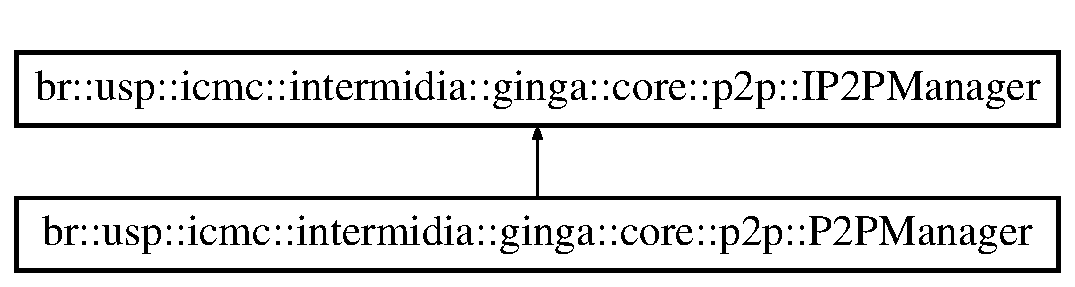
\includegraphics[height=2cm]{classbr_1_1usp_1_1icmc_1_1intermidia_1_1ginga_1_1core_1_1p2p_1_1IP2PManager}
\end{center}
\end{figure}
\subsection*{Tipos Públicos}
\begin{DoxyCompactItemize}
\item 
enum {\bf Status} \{ \par
{\bf NONE} =  0, 
{\bf OFFLINE} =  1, 
{\bf XA} =  2, 
{\bf AWAY} =  3, 
\par
{\bf DND} =  4, 
{\bf ONLINE} =  5, 
{\bf CHAT} =  6
 \}
\end{DoxyCompactItemize}
\subsection*{Métodos Públicos}
\begin{DoxyCompactItemize}
\item 
virtual {\bf $\sim$IP2PManager} ()
\item 
virtual void {\bf connect} (string server, int port, string username, talk\_\-base::InsecureCryptStringImpl pass, {\bf IP2PEventListener} $\ast$listener=NULL)=0
\item 
virtual void {\bf disconnect} ()=0
\item 
virtual void {\bf sendFiles} (vector$<$ string $>$ $\ast$files, string username)=0
\item 
virtual void {\bf sendFile} (string file, string username)=0
\item 
virtual void {\bf sendChatMessage} (string username, string text)=0
\item 
virtual vector$<$ buzz::Status $>$ $\ast$ {\bf getFriends} ()=0
\item 
virtual map$<$ string, buzz::Status $>$ $\ast$ {\bf getFriendsMap} ()=0
\item 
virtual void {\bf setStatus} ({\bf Status} s, string message)=0
\item 
virtual buzz::Status $\ast$ {\bf getStatus} ()=0
\item 
virtual void {\bf accept} ()=0
\item 
virtual void {\bf reject} ()=0
\end{DoxyCompactItemize}


\subsection{Descrição Detalhada}
Interface do gerenciador de conexões P2P. 

\subsection{Enumerações}
\index{br::usp::icmc::intermidia::ginga::core::p2p::IP2PManager@{br::usp::icmc::intermidia::ginga::core::p2p::IP2PManager}!Status@{Status}}
\index{Status@{Status}!br::usp::icmc::intermidia::ginga::core::p2p::IP2PManager@{br::usp::icmc::intermidia::ginga::core::p2p::IP2PManager}}
\subsubsection[{Status}]{\setlength{\rightskip}{0pt plus 5cm}enum {\bf br::usp::icmc::intermidia::ginga::core::p2p::IP2PManager::Status}}\label{classbr_1_1usp_1_1icmc_1_1intermidia_1_1ginga_1_1core_1_1p2p_1_1IP2PManager_ae4b55c6c0a7f1613e5616de08914237e}
\begin{Desc}
\item[Valores enumerados: ]\par
\begin{description}
\index{NONE@{NONE}!br::usp::icmc::intermidia::ginga::core::p2p::IP2PManager@{br::usp::icmc::intermidia::ginga::core::p2p::IP2PManager}}\index{br::usp::icmc::intermidia::ginga::core::p2p::IP2PManager@{br::usp::icmc::intermidia::ginga::core::p2p::IP2PManager}!NONE@{NONE}}\item[{\em 
NONE\label{classbr_1_1usp_1_1icmc_1_1intermidia_1_1ginga_1_1core_1_1p2p_1_1IP2PManager_ae4b55c6c0a7f1613e5616de08914237eab09a6a91504ac9afe2b5ba380172135c}
}]Usado quando o status não estiver definido. \index{OFFLINE@{OFFLINE}!br::usp::icmc::intermidia::ginga::core::p2p::IP2PManager@{br::usp::icmc::intermidia::ginga::core::p2p::IP2PManager}}\index{br::usp::icmc::intermidia::ginga::core::p2p::IP2PManager@{br::usp::icmc::intermidia::ginga::core::p2p::IP2PManager}!OFFLINE@{OFFLINE}}\item[{\em 
OFFLINE\label{classbr_1_1usp_1_1icmc_1_1intermidia_1_1ginga_1_1core_1_1p2p_1_1IP2PManager_ae4b55c6c0a7f1613e5616de08914237ea7461c990afc006337f7afee3a6a9e188}
}]Usado quando o usuário estiver desconectado. \index{XA@{XA}!br::usp::icmc::intermidia::ginga::core::p2p::IP2PManager@{br::usp::icmc::intermidia::ginga::core::p2p::IP2PManager}}\index{br::usp::icmc::intermidia::ginga::core::p2p::IP2PManager@{br::usp::icmc::intermidia::ginga::core::p2p::IP2PManager}!XA@{XA}}\item[{\em 
XA\label{classbr_1_1usp_1_1icmc_1_1intermidia_1_1ginga_1_1core_1_1p2p_1_1IP2PManager_ae4b55c6c0a7f1613e5616de08914237ea63b825d6fe1c817d7efda9a8d7147532}
}]eXtended Away -\/ Ausência estendida. \index{AWAY@{AWAY}!br::usp::icmc::intermidia::ginga::core::p2p::IP2PManager@{br::usp::icmc::intermidia::ginga::core::p2p::IP2PManager}}\index{br::usp::icmc::intermidia::ginga::core::p2p::IP2PManager@{br::usp::icmc::intermidia::ginga::core::p2p::IP2PManager}!AWAY@{AWAY}}\item[{\em 
AWAY\label{classbr_1_1usp_1_1icmc_1_1intermidia_1_1ginga_1_1core_1_1p2p_1_1IP2PManager_ae4b55c6c0a7f1613e5616de08914237ea05723d382e712227f615f55123684ea0}
}]Ausente \index{DND@{DND}!br::usp::icmc::intermidia::ginga::core::p2p::IP2PManager@{br::usp::icmc::intermidia::ginga::core::p2p::IP2PManager}}\index{br::usp::icmc::intermidia::ginga::core::p2p::IP2PManager@{br::usp::icmc::intermidia::ginga::core::p2p::IP2PManager}!DND@{DND}}\item[{\em 
DND\label{classbr_1_1usp_1_1icmc_1_1intermidia_1_1ginga_1_1core_1_1p2p_1_1IP2PManager_ae4b55c6c0a7f1613e5616de08914237eae7f30a061277349987d27d5785be55eb}
}]Do Not Disturb -\/ Não pertube. \index{ONLINE@{ONLINE}!br::usp::icmc::intermidia::ginga::core::p2p::IP2PManager@{br::usp::icmc::intermidia::ginga::core::p2p::IP2PManager}}\index{br::usp::icmc::intermidia::ginga::core::p2p::IP2PManager@{br::usp::icmc::intermidia::ginga::core::p2p::IP2PManager}!ONLINE@{ONLINE}}\item[{\em 
ONLINE\label{classbr_1_1usp_1_1icmc_1_1intermidia_1_1ginga_1_1core_1_1p2p_1_1IP2PManager_ae4b55c6c0a7f1613e5616de08914237ea637e72c86a809aed5430d4f554d4edfd}
}]Disponível. \index{CHAT@{CHAT}!br::usp::icmc::intermidia::ginga::core::p2p::IP2PManager@{br::usp::icmc::intermidia::ginga::core::p2p::IP2PManager}}\index{br::usp::icmc::intermidia::ginga::core::p2p::IP2PManager@{br::usp::icmc::intermidia::ginga::core::p2p::IP2PManager}!CHAT@{CHAT}}\item[{\em 
CHAT\label{classbr_1_1usp_1_1icmc_1_1intermidia_1_1ginga_1_1core_1_1p2p_1_1IP2PManager_ae4b55c6c0a7f1613e5616de08914237ea78f3642b5e139385a31bf83b14c3ce3d}
}]Querendo conversar. \end{description}
\end{Desc}



\subsection{Construtores \& Destrutores}
\index{br::usp::icmc::intermidia::ginga::core::p2p::IP2PManager@{br::usp::icmc::intermidia::ginga::core::p2p::IP2PManager}!$\sim$IP2PManager@{$\sim$IP2PManager}}
\index{$\sim$IP2PManager@{$\sim$IP2PManager}!br::usp::icmc::intermidia::ginga::core::p2p::IP2PManager@{br::usp::icmc::intermidia::ginga::core::p2p::IP2PManager}}
\subsubsection[{$\sim$IP2PManager}]{\setlength{\rightskip}{0pt plus 5cm}virtual br::usp::icmc::intermidia::ginga::core::p2p::IP2PManager::$\sim$IP2PManager ()\hspace{0.3cm}{\ttfamily  [inline, virtual]}}\label{classbr_1_1usp_1_1icmc_1_1intermidia_1_1ginga_1_1core_1_1p2p_1_1IP2PManager_a0601bca0990ec599cec1a5ed33cf9358}
Destói o objeto \doxyref{P2PManager}{pag.}{classbr_1_1usp_1_1icmc_1_1intermidia_1_1ginga_1_1core_1_1p2p_1_1P2PManager}. 

\subsection{Métodos}
\index{br::usp::icmc::intermidia::ginga::core::p2p::IP2PManager@{br::usp::icmc::intermidia::ginga::core::p2p::IP2PManager}!accept@{accept}}
\index{accept@{accept}!br::usp::icmc::intermidia::ginga::core::p2p::IP2PManager@{br::usp::icmc::intermidia::ginga::core::p2p::IP2PManager}}
\subsubsection[{accept}]{\setlength{\rightskip}{0pt plus 5cm}virtual void br::usp::icmc::intermidia::ginga::core::p2p::IP2PManager::accept ()\hspace{0.3cm}{\ttfamily  [pure virtual]}}\label{classbr_1_1usp_1_1icmc_1_1intermidia_1_1ginga_1_1core_1_1p2p_1_1IP2PManager_a2dcaff706e7b9f04602de239b287906d}
Aceita o recebimento de um arquivo. 

Implementado por {\bf br::usp::icmc::intermidia::ginga::core::p2p::P2PManager} \doxyref{}{pag.}{classbr_1_1usp_1_1icmc_1_1intermidia_1_1ginga_1_1core_1_1p2p_1_1P2PManager_a517504ad3a8bda8e3d76b5da7ba9939f}.

\index{br::usp::icmc::intermidia::ginga::core::p2p::IP2PManager@{br::usp::icmc::intermidia::ginga::core::p2p::IP2PManager}!connect@{connect}}
\index{connect@{connect}!br::usp::icmc::intermidia::ginga::core::p2p::IP2PManager@{br::usp::icmc::intermidia::ginga::core::p2p::IP2PManager}}
\subsubsection[{connect}]{\setlength{\rightskip}{0pt plus 5cm}virtual void br::usp::icmc::intermidia::ginga::core::p2p::IP2PManager::connect (string {\em server}, \/  int {\em port}, \/  string {\em username}, \/  talk\_\-base::InsecureCryptStringImpl {\em pass}, \/  {\bf IP2PEventListener} $\ast$ {\em listener} = {\ttfamily NULL})\hspace{0.3cm}{\ttfamily  [pure virtual]}}\label{classbr_1_1usp_1_1icmc_1_1intermidia_1_1ginga_1_1core_1_1p2p_1_1IP2PManager_a720d5e610e2018254d2ecc0237a9d4c4}
Conecta ao servidor/porta desejados usando o nome de usuário e senha fornecidos.


\begin{DoxyParams}{Parâmetros}
\item[{\em server}]Servidor a ser conectado. \item[{\em port}]Porta usada para conexão com servidor. \item[{\em username}]Nome do usuário utilizado na conexão. \item[{\em pass}]Senha utilizado na conexão. \item[{\em listener}]Observador de eventos relacionados à conexão P2P, como mudança do estado da conexão e de transferências de arquivos ou mudança de status de algum amigo. \end{DoxyParams}


Implementado por {\bf br::usp::icmc::intermidia::ginga::core::p2p::P2PManager} \doxyref{}{pag.}{classbr_1_1usp_1_1icmc_1_1intermidia_1_1ginga_1_1core_1_1p2p_1_1P2PManager_a8def9c0c69b0065372cdff8e558f17f4}.

\index{br::usp::icmc::intermidia::ginga::core::p2p::IP2PManager@{br::usp::icmc::intermidia::ginga::core::p2p::IP2PManager}!disconnect@{disconnect}}
\index{disconnect@{disconnect}!br::usp::icmc::intermidia::ginga::core::p2p::IP2PManager@{br::usp::icmc::intermidia::ginga::core::p2p::IP2PManager}}
\subsubsection[{disconnect}]{\setlength{\rightskip}{0pt plus 5cm}virtual void br::usp::icmc::intermidia::ginga::core::p2p::IP2PManager::disconnect ()\hspace{0.3cm}{\ttfamily  [pure virtual]}}\label{classbr_1_1usp_1_1icmc_1_1intermidia_1_1ginga_1_1core_1_1p2p_1_1IP2PManager_a48b9e24798125b0937abdb1577475991}
Disconecta do servidor. 

Implementado por {\bf br::usp::icmc::intermidia::ginga::core::p2p::P2PManager} \doxyref{}{pag.}{classbr_1_1usp_1_1icmc_1_1intermidia_1_1ginga_1_1core_1_1p2p_1_1P2PManager_a52a7440c36acc668ae0dba42edd67b7d}.

\index{br::usp::icmc::intermidia::ginga::core::p2p::IP2PManager@{br::usp::icmc::intermidia::ginga::core::p2p::IP2PManager}!getFriends@{getFriends}}
\index{getFriends@{getFriends}!br::usp::icmc::intermidia::ginga::core::p2p::IP2PManager@{br::usp::icmc::intermidia::ginga::core::p2p::IP2PManager}}
\subsubsection[{getFriends}]{\setlength{\rightskip}{0pt plus 5cm}virtual vector$<$buzz::Status$>$$\ast$ br::usp::icmc::intermidia::ginga::core::p2p::IP2PManager::getFriends ()\hspace{0.3cm}{\ttfamily  [pure virtual]}}\label{classbr_1_1usp_1_1icmc_1_1intermidia_1_1ginga_1_1core_1_1p2p_1_1IP2PManager_a45c81b565c3112b7d37328103f0918ab}
Retorna a lista de amigos conectados.

\begin{DoxyReturn}{Retorna}
Um vetor com o status dos amigos conectados. completo. 
\end{DoxyReturn}


Implementado por {\bf br::usp::icmc::intermidia::ginga::core::p2p::P2PManager} \doxyref{}{pag.}{classbr_1_1usp_1_1icmc_1_1intermidia_1_1ginga_1_1core_1_1p2p_1_1P2PManager_ab67876af258af7547c489675afb93635}.

\index{br::usp::icmc::intermidia::ginga::core::p2p::IP2PManager@{br::usp::icmc::intermidia::ginga::core::p2p::IP2PManager}!getFriendsMap@{getFriendsMap}}
\index{getFriendsMap@{getFriendsMap}!br::usp::icmc::intermidia::ginga::core::p2p::IP2PManager@{br::usp::icmc::intermidia::ginga::core::p2p::IP2PManager}}
\subsubsection[{getFriendsMap}]{\setlength{\rightskip}{0pt plus 5cm}virtual map$<$string, buzz::Status$>$$\ast$ br::usp::icmc::intermidia::ginga::core::p2p::IP2PManager::getFriendsMap ()\hspace{0.3cm}{\ttfamily  [pure virtual]}}\label{classbr_1_1usp_1_1icmc_1_1intermidia_1_1ginga_1_1core_1_1p2p_1_1IP2PManager_abfa3890264dd16b4b9d9eec28d13f69e}
Retorna a lista de amigos conectados.

\begin{DoxyReturn}{Retorna}
Um mapa que relaciona o identificador do amigo (jid completo em forma de string) com seu status completo. 
\end{DoxyReturn}


Implementado por {\bf br::usp::icmc::intermidia::ginga::core::p2p::P2PManager} \doxyref{}{pag.}{classbr_1_1usp_1_1icmc_1_1intermidia_1_1ginga_1_1core_1_1p2p_1_1P2PManager_a878ba7b06d254deb977941a0f73cc81c}.

\index{br::usp::icmc::intermidia::ginga::core::p2p::IP2PManager@{br::usp::icmc::intermidia::ginga::core::p2p::IP2PManager}!getStatus@{getStatus}}
\index{getStatus@{getStatus}!br::usp::icmc::intermidia::ginga::core::p2p::IP2PManager@{br::usp::icmc::intermidia::ginga::core::p2p::IP2PManager}}
\subsubsection[{getStatus}]{\setlength{\rightskip}{0pt plus 5cm}virtual buzz::Status$\ast$ br::usp::icmc::intermidia::ginga::core::p2p::IP2PManager::getStatus ()\hspace{0.3cm}{\ttfamily  [pure virtual]}}\label{classbr_1_1usp_1_1icmc_1_1intermidia_1_1ginga_1_1core_1_1p2p_1_1IP2PManager_a3e566b2e50875009b254caeed5f374f9}
Permite acessar o próprio status. Pode ser chamado antes ou depois de se conectar.

\begin{DoxyReturn}{Retorna}
Status completo. 
\end{DoxyReturn}


Implementado por {\bf br::usp::icmc::intermidia::ginga::core::p2p::P2PManager} \doxyref{}{pag.}{classbr_1_1usp_1_1icmc_1_1intermidia_1_1ginga_1_1core_1_1p2p_1_1P2PManager_a034857fb3348c52ec13fe66f8ee1fb3c}.

\index{br::usp::icmc::intermidia::ginga::core::p2p::IP2PManager@{br::usp::icmc::intermidia::ginga::core::p2p::IP2PManager}!reject@{reject}}
\index{reject@{reject}!br::usp::icmc::intermidia::ginga::core::p2p::IP2PManager@{br::usp::icmc::intermidia::ginga::core::p2p::IP2PManager}}
\subsubsection[{reject}]{\setlength{\rightskip}{0pt plus 5cm}virtual void br::usp::icmc::intermidia::ginga::core::p2p::IP2PManager::reject ()\hspace{0.3cm}{\ttfamily  [pure virtual]}}\label{classbr_1_1usp_1_1icmc_1_1intermidia_1_1ginga_1_1core_1_1p2p_1_1IP2PManager_ac43a21a8308ca36d1143026bbca1a4a9}
Rejeita o recebimento de um arquivo. 

Implementado por {\bf br::usp::icmc::intermidia::ginga::core::p2p::P2PManager} \doxyref{}{pag.}{classbr_1_1usp_1_1icmc_1_1intermidia_1_1ginga_1_1core_1_1p2p_1_1P2PManager_a891a4047a8955c761683eecced70a43d}.

\index{br::usp::icmc::intermidia::ginga::core::p2p::IP2PManager@{br::usp::icmc::intermidia::ginga::core::p2p::IP2PManager}!sendChatMessage@{sendChatMessage}}
\index{sendChatMessage@{sendChatMessage}!br::usp::icmc::intermidia::ginga::core::p2p::IP2PManager@{br::usp::icmc::intermidia::ginga::core::p2p::IP2PManager}}
\subsubsection[{sendChatMessage}]{\setlength{\rightskip}{0pt plus 5cm}virtual void br::usp::icmc::intermidia::ginga::core::p2p::IP2PManager::sendChatMessage (string {\em username}, \/  string {\em text})\hspace{0.3cm}{\ttfamily  [pure virtual]}}\label{classbr_1_1usp_1_1icmc_1_1intermidia_1_1ginga_1_1core_1_1p2p_1_1IP2PManager_a4de46a01e59fd8986ee7ccee739e49a1}
Envia uma mensagem de texto para um determinado amigo.


\begin{DoxyParams}{Parâmetros}
\item[{\em username}]Identificador o amigo que irá receber os arquivos \item[{\em text}]Mensagem a ser enviada \end{DoxyParams}


Implementado por {\bf br::usp::icmc::intermidia::ginga::core::p2p::P2PManager} \doxyref{}{pag.}{classbr_1_1usp_1_1icmc_1_1intermidia_1_1ginga_1_1core_1_1p2p_1_1P2PManager_aba42f2f112f2cf40bb06d4ab5e91cbc1}.

\index{br::usp::icmc::intermidia::ginga::core::p2p::IP2PManager@{br::usp::icmc::intermidia::ginga::core::p2p::IP2PManager}!sendFile@{sendFile}}
\index{sendFile@{sendFile}!br::usp::icmc::intermidia::ginga::core::p2p::IP2PManager@{br::usp::icmc::intermidia::ginga::core::p2p::IP2PManager}}
\subsubsection[{sendFile}]{\setlength{\rightskip}{0pt plus 5cm}virtual void br::usp::icmc::intermidia::ginga::core::p2p::IP2PManager::sendFile (string {\em file}, \/  string {\em username})\hspace{0.3cm}{\ttfamily  [pure virtual]}}\label{classbr_1_1usp_1_1icmc_1_1intermidia_1_1ginga_1_1core_1_1p2p_1_1IP2PManager_a780b05d26f8438b405cc176051ab31f4}
Envia arquivo ou diretório para um determinado amigo.


\begin{DoxyParams}{Parâmetros}
\item[{\em file}]Caminho do arquivo ou diretório que será enviado \item[{\em jid}]Identificador o amigo que irá receber os arquivos \end{DoxyParams}


Implementado por {\bf br::usp::icmc::intermidia::ginga::core::p2p::P2PManager} \doxyref{}{pag.}{classbr_1_1usp_1_1icmc_1_1intermidia_1_1ginga_1_1core_1_1p2p_1_1P2PManager_a9fb02062e8400eef048133a547d9b5fa}.

\index{br::usp::icmc::intermidia::ginga::core::p2p::IP2PManager@{br::usp::icmc::intermidia::ginga::core::p2p::IP2PManager}!sendFiles@{sendFiles}}
\index{sendFiles@{sendFiles}!br::usp::icmc::intermidia::ginga::core::p2p::IP2PManager@{br::usp::icmc::intermidia::ginga::core::p2p::IP2PManager}}
\subsubsection[{sendFiles}]{\setlength{\rightskip}{0pt plus 5cm}virtual void br::usp::icmc::intermidia::ginga::core::p2p::IP2PManager::sendFiles (vector$<$ string $>$ $\ast$ {\em files}, \/  string {\em username})\hspace{0.3cm}{\ttfamily  [pure virtual]}}\label{classbr_1_1usp_1_1icmc_1_1intermidia_1_1ginga_1_1core_1_1p2p_1_1IP2PManager_a5d90e6289098fedff8131f6a31e6be18}
Envia arquivos e diretórios para um determinado amigo.


\begin{DoxyParams}{Parâmetros}
\item[{\em files}]Vetor contendo os caminhos dos arquivos e diretórios que serão enviados \item[{\em jid}]Identificador o amigo que irá receber os arquivos \end{DoxyParams}


Implementado por {\bf br::usp::icmc::intermidia::ginga::core::p2p::P2PManager} \doxyref{}{pag.}{classbr_1_1usp_1_1icmc_1_1intermidia_1_1ginga_1_1core_1_1p2p_1_1P2PManager_abcf62501438880b04515606c80939c9e}.

\index{br::usp::icmc::intermidia::ginga::core::p2p::IP2PManager@{br::usp::icmc::intermidia::ginga::core::p2p::IP2PManager}!setStatus@{setStatus}}
\index{setStatus@{setStatus}!br::usp::icmc::intermidia::ginga::core::p2p::IP2PManager@{br::usp::icmc::intermidia::ginga::core::p2p::IP2PManager}}
\subsubsection[{setStatus}]{\setlength{\rightskip}{0pt plus 5cm}virtual void br::usp::icmc::intermidia::ginga::core::p2p::IP2PManager::setStatus ({\bf Status} {\em s}, \/  string {\em message})\hspace{0.3cm}{\ttfamily  [pure virtual]}}\label{classbr_1_1usp_1_1icmc_1_1intermidia_1_1ginga_1_1core_1_1p2p_1_1IP2PManager_adc2163d5ef7493c9d23f74a7fcdbb398}
Permite definir o próprio status. Pode ser chamado antes ou depois de se conectar.


\begin{DoxyParams}{Parâmetros}
\item[{\em s}]Status a ser utilizado. \end{DoxyParams}
\begin{DoxySeeAlso}{Veja também}
\doxyref{Status}{pag.}{classbr_1_1usp_1_1icmc_1_1intermidia_1_1ginga_1_1core_1_1p2p_1_1IP2PManager_ae4b55c6c0a7f1613e5616de08914237e}. 
\end{DoxySeeAlso}

\begin{DoxyParams}{Parâmetros}
\item[{\em message}]Mensagem personalizada opcional. \end{DoxyParams}


Implementado por {\bf br::usp::icmc::intermidia::ginga::core::p2p::P2PManager} \doxyref{}{pag.}{classbr_1_1usp_1_1icmc_1_1intermidia_1_1ginga_1_1core_1_1p2p_1_1P2PManager_acdeac6f81a5606acf66cfe9b0de46994}.



A documentação para esta classe foi gerada a partir do seguinte arquivo:\begin{DoxyCompactItemize}
\item 
include/{\bf IP2PManager.h}\end{DoxyCompactItemize}

\section{Referência da Classe br::usp::icmc::intermidia::ginga::core::p2p::P2PManager}
\label{classbr_1_1usp_1_1icmc_1_1intermidia_1_1ginga_1_1core_1_1p2p_1_1P2PManager}\index{br::usp::icmc::intermidia::ginga::core::p2p::P2PManager@{br::usp::icmc::intermidia::ginga::core::p2p::P2PManager}}


{\ttfamily \#include $<$P2PManager.h$>$}

Diagrama de Hierarquia para br::usp::icmc::intermidia::ginga::core::p2p::P2PManager:\begin{figure}[H]
\begin{center}
\leavevmode
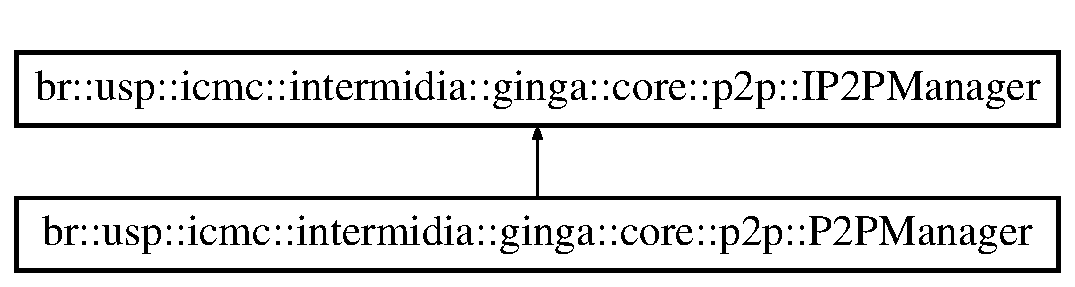
\includegraphics[height=2cm]{classbr_1_1usp_1_1icmc_1_1intermidia_1_1ginga_1_1core_1_1p2p_1_1P2PManager}
\end{center}
\end{figure}
\subsection*{Métodos Públicos}
\begin{DoxyCompactItemize}
\item 
{\bf P2PManager} ()
\item 
virtual {\bf $\sim$P2PManager} ()
\item 
void {\bf connect} (string server, int port, string username, talk\_\-base::InsecureCryptStringImpl pass, {\bf IP2PEventListener} $\ast$listener=NULL)
\item 
void {\bf disconnect} ()
\item 
void {\bf sendFiles} (vector$<$ string $>$ $\ast$files, string username)
\item 
void {\bf sendFile} (string file, string username)
\item 
void {\bf sendChatMessage} (string username, string text)
\item 
vector$<$ buzz::Status $>$ $\ast$ {\bf getFriends} ()
\item 
map$<$ string, buzz::Status $>$ $\ast$ {\bf getFriendsMap} ()
\item 
void {\bf setStatus} ({\bf Status} s, string mensagem)
\item 
buzz::Status $\ast$ {\bf getStatus} ()
\item 
void {\bf accept} ()
\item 
void {\bf reject} ()
\end{DoxyCompactItemize}


\subsection{Descrição Detalhada}
Classe responsável por gerenciar conexões P2P. 

\subsection{Construtores \& Destrutores}
\index{br::usp::icmc::intermidia::ginga::core::p2p::P2PManager@{br::usp::icmc::intermidia::ginga::core::p2p::P2PManager}!P2PManager@{P2PManager}}
\index{P2PManager@{P2PManager}!br::usp::icmc::intermidia::ginga::core::p2p::P2PManager@{br::usp::icmc::intermidia::ginga::core::p2p::P2PManager}}
\subsubsection[{P2PManager}]{\setlength{\rightskip}{0pt plus 5cm}br::usp::icmc::intermidia::ginga::core::p2p::P2PManager::P2PManager ()}\label{classbr_1_1usp_1_1icmc_1_1intermidia_1_1ginga_1_1core_1_1p2p_1_1P2PManager_a56fc2a96c4831da31bd6f63fdb37f9e6}
Constrói um objeto \doxyref{P2PManager}{pag.}{classbr_1_1usp_1_1icmc_1_1intermidia_1_1ginga_1_1core_1_1p2p_1_1P2PManager}. \index{br::usp::icmc::intermidia::ginga::core::p2p::P2PManager@{br::usp::icmc::intermidia::ginga::core::p2p::P2PManager}!$\sim$P2PManager@{$\sim$P2PManager}}
\index{$\sim$P2PManager@{$\sim$P2PManager}!br::usp::icmc::intermidia::ginga::core::p2p::P2PManager@{br::usp::icmc::intermidia::ginga::core::p2p::P2PManager}}
\subsubsection[{$\sim$P2PManager}]{\setlength{\rightskip}{0pt plus 5cm}br::usp::icmc::intermidia::ginga::core::p2p::P2PManager::$\sim$P2PManager ()\hspace{0.3cm}{\ttfamily  [virtual]}}\label{classbr_1_1usp_1_1icmc_1_1intermidia_1_1ginga_1_1core_1_1p2p_1_1P2PManager_a79b95dc9eb7c0d148a3f03990e5f49b6}
Destói o objeto \doxyref{P2PManager}{pag.}{classbr_1_1usp_1_1icmc_1_1intermidia_1_1ginga_1_1core_1_1p2p_1_1P2PManager}. 

\subsection{Métodos}
\index{br::usp::icmc::intermidia::ginga::core::p2p::P2PManager@{br::usp::icmc::intermidia::ginga::core::p2p::P2PManager}!accept@{accept}}
\index{accept@{accept}!br::usp::icmc::intermidia::ginga::core::p2p::P2PManager@{br::usp::icmc::intermidia::ginga::core::p2p::P2PManager}}
\subsubsection[{accept}]{\setlength{\rightskip}{0pt plus 5cm}void br::usp::icmc::intermidia::ginga::core::p2p::P2PManager::accept ()\hspace{0.3cm}{\ttfamily  [virtual]}}\label{classbr_1_1usp_1_1icmc_1_1intermidia_1_1ginga_1_1core_1_1p2p_1_1P2PManager_a517504ad3a8bda8e3d76b5da7ba9939f}
Aceita o recebimento de um arquivo. 

Implementa {\bf br::usp::icmc::intermidia::ginga::core::p2p::IP2PManager} \doxyref{}{pag.}{classbr_1_1usp_1_1icmc_1_1intermidia_1_1ginga_1_1core_1_1p2p_1_1IP2PManager_a2dcaff706e7b9f04602de239b287906d}.

\index{br::usp::icmc::intermidia::ginga::core::p2p::P2PManager@{br::usp::icmc::intermidia::ginga::core::p2p::P2PManager}!connect@{connect}}
\index{connect@{connect}!br::usp::icmc::intermidia::ginga::core::p2p::P2PManager@{br::usp::icmc::intermidia::ginga::core::p2p::P2PManager}}
\subsubsection[{connect}]{\setlength{\rightskip}{0pt plus 5cm}void br::usp::icmc::intermidia::ginga::core::p2p::P2PManager::connect (string {\em server}, \/  int {\em port}, \/  string {\em username}, \/  talk\_\-base::InsecureCryptStringImpl {\em pass}, \/  {\bf IP2PEventListener} $\ast$ {\em listener} = {\ttfamily NULL})\hspace{0.3cm}{\ttfamily  [virtual]}}\label{classbr_1_1usp_1_1icmc_1_1intermidia_1_1ginga_1_1core_1_1p2p_1_1P2PManager_a8def9c0c69b0065372cdff8e558f17f4}
Conecta ao servidor/porta desejados usando o nome de usuário e senha fornecidos.


\begin{DoxyParams}{Parâmetros}
\item[{\em server}]Servidor a ser conectado. \item[{\em port}]Porta usada para conexão com servidor. \item[{\em username}]Nome do usuário utilizado na conexão. \item[{\em pass}]Senha utilizado na conexão. \item[{\em listener}]Observador de eventos relacionados à conexão P2P, como mudança do estado da conexão e de transferências de arquivos ou mudança de status de algum amigo. \end{DoxyParams}


Implementa {\bf br::usp::icmc::intermidia::ginga::core::p2p::IP2PManager} \doxyref{}{pag.}{classbr_1_1usp_1_1icmc_1_1intermidia_1_1ginga_1_1core_1_1p2p_1_1IP2PManager_a720d5e610e2018254d2ecc0237a9d4c4}.

\index{br::usp::icmc::intermidia::ginga::core::p2p::P2PManager@{br::usp::icmc::intermidia::ginga::core::p2p::P2PManager}!disconnect@{disconnect}}
\index{disconnect@{disconnect}!br::usp::icmc::intermidia::ginga::core::p2p::P2PManager@{br::usp::icmc::intermidia::ginga::core::p2p::P2PManager}}
\subsubsection[{disconnect}]{\setlength{\rightskip}{0pt plus 5cm}void br::usp::icmc::intermidia::ginga::core::p2p::P2PManager::disconnect ()\hspace{0.3cm}{\ttfamily  [virtual]}}\label{classbr_1_1usp_1_1icmc_1_1intermidia_1_1ginga_1_1core_1_1p2p_1_1P2PManager_a52a7440c36acc668ae0dba42edd67b7d}
Disconecta do servidor. 

Implementa {\bf br::usp::icmc::intermidia::ginga::core::p2p::IP2PManager} \doxyref{}{pag.}{classbr_1_1usp_1_1icmc_1_1intermidia_1_1ginga_1_1core_1_1p2p_1_1IP2PManager_a48b9e24798125b0937abdb1577475991}.

\index{br::usp::icmc::intermidia::ginga::core::p2p::P2PManager@{br::usp::icmc::intermidia::ginga::core::p2p::P2PManager}!getFriends@{getFriends}}
\index{getFriends@{getFriends}!br::usp::icmc::intermidia::ginga::core::p2p::P2PManager@{br::usp::icmc::intermidia::ginga::core::p2p::P2PManager}}
\subsubsection[{getFriends}]{\setlength{\rightskip}{0pt plus 5cm}vector$<$ buzz::Status $>$ $\ast$ br::usp::icmc::intermidia::ginga::core::p2p::P2PManager::getFriends ()\hspace{0.3cm}{\ttfamily  [virtual]}}\label{classbr_1_1usp_1_1icmc_1_1intermidia_1_1ginga_1_1core_1_1p2p_1_1P2PManager_ab67876af258af7547c489675afb93635}
Retorna a lista de amigos conectados.

\begin{DoxyReturn}{Retorna}
Um vetor com o status dos amigos conectados. completo. 
\end{DoxyReturn}


Implementa {\bf br::usp::icmc::intermidia::ginga::core::p2p::IP2PManager} \doxyref{}{pag.}{classbr_1_1usp_1_1icmc_1_1intermidia_1_1ginga_1_1core_1_1p2p_1_1IP2PManager_a45c81b565c3112b7d37328103f0918ab}.

\index{br::usp::icmc::intermidia::ginga::core::p2p::P2PManager@{br::usp::icmc::intermidia::ginga::core::p2p::P2PManager}!getFriendsMap@{getFriendsMap}}
\index{getFriendsMap@{getFriendsMap}!br::usp::icmc::intermidia::ginga::core::p2p::P2PManager@{br::usp::icmc::intermidia::ginga::core::p2p::P2PManager}}
\subsubsection[{getFriendsMap}]{\setlength{\rightskip}{0pt plus 5cm}map$<$ string, buzz::Status $>$ $\ast$ br::usp::icmc::intermidia::ginga::core::p2p::P2PManager::getFriendsMap ()\hspace{0.3cm}{\ttfamily  [virtual]}}\label{classbr_1_1usp_1_1icmc_1_1intermidia_1_1ginga_1_1core_1_1p2p_1_1P2PManager_a878ba7b06d254deb977941a0f73cc81c}
Retorna a lista de amigos conectados.

\begin{DoxyReturn}{Retorna}
Um mapa que relaciona o identificador do amigo (jid completo em forma de string) com seu status completo. 
\end{DoxyReturn}


Implementa {\bf br::usp::icmc::intermidia::ginga::core::p2p::IP2PManager} \doxyref{}{pag.}{classbr_1_1usp_1_1icmc_1_1intermidia_1_1ginga_1_1core_1_1p2p_1_1IP2PManager_abfa3890264dd16b4b9d9eec28d13f69e}.

\index{br::usp::icmc::intermidia::ginga::core::p2p::P2PManager@{br::usp::icmc::intermidia::ginga::core::p2p::P2PManager}!getStatus@{getStatus}}
\index{getStatus@{getStatus}!br::usp::icmc::intermidia::ginga::core::p2p::P2PManager@{br::usp::icmc::intermidia::ginga::core::p2p::P2PManager}}
\subsubsection[{getStatus}]{\setlength{\rightskip}{0pt plus 5cm}buzz::Status $\ast$ br::usp::icmc::intermidia::ginga::core::p2p::P2PManager::getStatus ()\hspace{0.3cm}{\ttfamily  [virtual]}}\label{classbr_1_1usp_1_1icmc_1_1intermidia_1_1ginga_1_1core_1_1p2p_1_1P2PManager_a034857fb3348c52ec13fe66f8ee1fb3c}
Permite acessar o próprio status. Pode ser chamado antes ou depois de se conectar.

\begin{DoxyReturn}{Retorna}
Status completo. 
\end{DoxyReturn}


Implementa {\bf br::usp::icmc::intermidia::ginga::core::p2p::IP2PManager} \doxyref{}{pag.}{classbr_1_1usp_1_1icmc_1_1intermidia_1_1ginga_1_1core_1_1p2p_1_1IP2PManager_a3e566b2e50875009b254caeed5f374f9}.

\index{br::usp::icmc::intermidia::ginga::core::p2p::P2PManager@{br::usp::icmc::intermidia::ginga::core::p2p::P2PManager}!reject@{reject}}
\index{reject@{reject}!br::usp::icmc::intermidia::ginga::core::p2p::P2PManager@{br::usp::icmc::intermidia::ginga::core::p2p::P2PManager}}
\subsubsection[{reject}]{\setlength{\rightskip}{0pt plus 5cm}void br::usp::icmc::intermidia::ginga::core::p2p::P2PManager::reject ()\hspace{0.3cm}{\ttfamily  [virtual]}}\label{classbr_1_1usp_1_1icmc_1_1intermidia_1_1ginga_1_1core_1_1p2p_1_1P2PManager_a891a4047a8955c761683eecced70a43d}
Rejeita o recebimento de um arquivo. 

Implementa {\bf br::usp::icmc::intermidia::ginga::core::p2p::IP2PManager} \doxyref{}{pag.}{classbr_1_1usp_1_1icmc_1_1intermidia_1_1ginga_1_1core_1_1p2p_1_1IP2PManager_ac43a21a8308ca36d1143026bbca1a4a9}.

\index{br::usp::icmc::intermidia::ginga::core::p2p::P2PManager@{br::usp::icmc::intermidia::ginga::core::p2p::P2PManager}!sendChatMessage@{sendChatMessage}}
\index{sendChatMessage@{sendChatMessage}!br::usp::icmc::intermidia::ginga::core::p2p::P2PManager@{br::usp::icmc::intermidia::ginga::core::p2p::P2PManager}}
\subsubsection[{sendChatMessage}]{\setlength{\rightskip}{0pt plus 5cm}void br::usp::icmc::intermidia::ginga::core::p2p::P2PManager::sendChatMessage (string {\em username}, \/  string {\em text})\hspace{0.3cm}{\ttfamily  [virtual]}}\label{classbr_1_1usp_1_1icmc_1_1intermidia_1_1ginga_1_1core_1_1p2p_1_1P2PManager_aba42f2f112f2cf40bb06d4ab5e91cbc1}
Envia uma mensagem de texto para um determinado amigo.


\begin{DoxyParams}{Parâmetros}
\item[{\em username}]Identificador o amigo que irá receber os arquivos \item[{\em text}]Mensagem a ser enviada \end{DoxyParams}


Implementa {\bf br::usp::icmc::intermidia::ginga::core::p2p::IP2PManager} \doxyref{}{pag.}{classbr_1_1usp_1_1icmc_1_1intermidia_1_1ginga_1_1core_1_1p2p_1_1IP2PManager_a4de46a01e59fd8986ee7ccee739e49a1}.

\index{br::usp::icmc::intermidia::ginga::core::p2p::P2PManager@{br::usp::icmc::intermidia::ginga::core::p2p::P2PManager}!sendFile@{sendFile}}
\index{sendFile@{sendFile}!br::usp::icmc::intermidia::ginga::core::p2p::P2PManager@{br::usp::icmc::intermidia::ginga::core::p2p::P2PManager}}
\subsubsection[{sendFile}]{\setlength{\rightskip}{0pt plus 5cm}void br::usp::icmc::intermidia::ginga::core::p2p::P2PManager::sendFile (string {\em file}, \/  string {\em username})\hspace{0.3cm}{\ttfamily  [virtual]}}\label{classbr_1_1usp_1_1icmc_1_1intermidia_1_1ginga_1_1core_1_1p2p_1_1P2PManager_a9fb02062e8400eef048133a547d9b5fa}
Envia arquivo ou diretório para um determinado amigo.


\begin{DoxyParams}{Parâmetros}
\item[{\em file}]Caminho do arquivo ou diretório que será enviado \item[{\em jid}]Identificador o amigo que irá receber os arquivos \end{DoxyParams}


Implementa {\bf br::usp::icmc::intermidia::ginga::core::p2p::IP2PManager} \doxyref{}{pag.}{classbr_1_1usp_1_1icmc_1_1intermidia_1_1ginga_1_1core_1_1p2p_1_1IP2PManager_a780b05d26f8438b405cc176051ab31f4}.

\index{br::usp::icmc::intermidia::ginga::core::p2p::P2PManager@{br::usp::icmc::intermidia::ginga::core::p2p::P2PManager}!sendFiles@{sendFiles}}
\index{sendFiles@{sendFiles}!br::usp::icmc::intermidia::ginga::core::p2p::P2PManager@{br::usp::icmc::intermidia::ginga::core::p2p::P2PManager}}
\subsubsection[{sendFiles}]{\setlength{\rightskip}{0pt plus 5cm}void br::usp::icmc::intermidia::ginga::core::p2p::P2PManager::sendFiles (vector$<$ string $>$ $\ast$ {\em files}, \/  string {\em username})\hspace{0.3cm}{\ttfamily  [virtual]}}\label{classbr_1_1usp_1_1icmc_1_1intermidia_1_1ginga_1_1core_1_1p2p_1_1P2PManager_abcf62501438880b04515606c80939c9e}
Envia arquivos e diretórios para um determinado amigo.


\begin{DoxyParams}{Parâmetros}
\item[{\em files}]Vetor contendo os caminhos dos arquivos e diretórios que serão enviados \item[{\em username}]Identificador o amigo que irá receber os arquivos \end{DoxyParams}


Implementa {\bf br::usp::icmc::intermidia::ginga::core::p2p::IP2PManager} \doxyref{}{pag.}{classbr_1_1usp_1_1icmc_1_1intermidia_1_1ginga_1_1core_1_1p2p_1_1IP2PManager_a5d90e6289098fedff8131f6a31e6be18}.

\index{br::usp::icmc::intermidia::ginga::core::p2p::P2PManager@{br::usp::icmc::intermidia::ginga::core::p2p::P2PManager}!setStatus@{setStatus}}
\index{setStatus@{setStatus}!br::usp::icmc::intermidia::ginga::core::p2p::P2PManager@{br::usp::icmc::intermidia::ginga::core::p2p::P2PManager}}
\subsubsection[{setStatus}]{\setlength{\rightskip}{0pt plus 5cm}void br::usp::icmc::intermidia::ginga::core::p2p::P2PManager::setStatus ({\bf Status} {\em s}, \/  string {\em mensagem})\hspace{0.3cm}{\ttfamily  [virtual]}}\label{classbr_1_1usp_1_1icmc_1_1intermidia_1_1ginga_1_1core_1_1p2p_1_1P2PManager_acdeac6f81a5606acf66cfe9b0de46994}
Permite definir o próprio status. Pode ser chamado antes ou depois de se conectar.


\begin{DoxyParams}{Parâmetros}
\item[{\em s}]Status a ser utilizado. \end{DoxyParams}
\begin{DoxySeeAlso}{Veja também}
\doxyref{Status}{pag.}{classbr_1_1usp_1_1icmc_1_1intermidia_1_1ginga_1_1core_1_1p2p_1_1IP2PManager_ae4b55c6c0a7f1613e5616de08914237e}. 
\end{DoxySeeAlso}

\begin{DoxyParams}{Parâmetros}
\item[{\em message}]Mensagem personalizada opcional. \end{DoxyParams}


Implementa {\bf br::usp::icmc::intermidia::ginga::core::p2p::IP2PManager} \doxyref{}{pag.}{classbr_1_1usp_1_1icmc_1_1intermidia_1_1ginga_1_1core_1_1p2p_1_1IP2PManager_adc2163d5ef7493c9d23f74a7fcdbb398}.



A documentação para esta classe foi gerada a partir dos seguintes arquivos:\begin{DoxyCompactItemize}
\item 
include/{\bf P2PManager.h}\item 
src/{\bf P2PManager.cpp}\end{DoxyCompactItemize}

\chapter{Arquivos}
\section{Referência do Arquivo include/ChatTask.h}
\label{ChatTask_8h}\index{include/ChatTask.h@{include/ChatTask.h}}
{\ttfamily \#include $<$talk/xmpp/xmppengine.h$>$}\par
{\ttfamily \#include $<$talk/xmpp/xmpptask.h$>$}\par
{\ttfamily \#include $<$linceutil/LoggerUtil.h$>$}\par
\subsection*{Componentes}
\begin{DoxyCompactItemize}
\item 
class {\bf br::usp::icmc::intermidia::ginga::core::p2p::ChatTask}
\end{DoxyCompactItemize}


\subsection{Descrição Detalhada}
\begin{DoxyAuthor}{Autor}
Diogo de Carvalho Pedrosa 

José Augusto Costa Martins Júnior 
\end{DoxyAuthor}
\begin{DoxyDate}{Data}
10-\/08-\/10 
\end{DoxyDate}

\section{Referência do Arquivo include/FileShareClient.h}
\label{FileShareClient_8h}\index{include/FileShareClient.h@{include/FileShareClient.h}}
{\ttfamily \#include $<$talk/session/fileshare/fileshare.h$>$}\par
{\ttfamily \#include $<$talk/examples/login/status.h$>$}\par
{\ttfamily \#include $<$talk/xmpp/jid.h$>$}\par
{\ttfamily \#include $<$linceutil/LoggerUtil.h$>$}\par
\subsection*{Componentes}
\begin{DoxyCompactItemize}
\item 
class {\bf br::usp::icmc::intermidia::ginga::core::p2p::FileShareClient}
\end{DoxyCompactItemize}


\subsection{Descrição Detalhada}
\begin{DoxyAuthor}{Autor}
Armando Biagioni Neto 

Diogo de Carvalho Pedrosa 

José Augusto Costa Martins Júnior 
\end{DoxyAuthor}
\begin{DoxyDate}{Data}
22-\/07-\/10 
\end{DoxyDate}

\section{Referência do Arquivo include/IP2PEventListener.h}
\label{IP2PEventListener_8h}\index{include/IP2PEventListener.h@{include/IP2PEventListener.h}}
{\ttfamily \#include \char`\"{}FileShareClient.h\char`\"{}}\par
{\ttfamily \#include $<$talk/session/fileshare/fileshare.h$>$}\par
{\ttfamily \#include $<$talk/examples/login/status.h$>$}\par
{\ttfamily \#include $<$talk/xmpp/jid.h$>$}\par
{\ttfamily \#include $<$linceutil/LoggerUtil.h$>$}\par
{\ttfamily \#include $<$talk/xmpp/xmppengine.h$>$}\par
\subsection*{Componentes}
\begin{DoxyCompactItemize}
\item 
class {\bf br::usp::icmc::intermidia::ginga::core::p2p::IP2PEventListener}
\end{DoxyCompactItemize}


\subsection{Descrição Detalhada}
\begin{DoxyAuthor}{Autor}
Diogo de Carvalho Pedrosa 
\end{DoxyAuthor}
\begin{DoxyDate}{Data}
13-\/08-\/10 
\end{DoxyDate}

\section{Referência do Arquivo include/IP2PManager.h}
\label{IP2PManager_8h}\index{include/IP2PManager.h@{include/IP2PManager.h}}
{\ttfamily \#include $<$string$>$}\par
{\ttfamily \#include $<$vector$>$}\par
{\ttfamily \#include \char`\"{}IP2PEventListener.h\char`\"{}}\par
{\ttfamily \#include \char`\"{}FileShareClient.h\char`\"{}}\par
{\ttfamily \#include $<$talk/xmpp/xmppengine.h$>$}\par
{\ttfamily \#include $<$talk/base/cryptstring.h$>$}\par
{\ttfamily \#include $<$talk/examples/login/status.h$>$}\par
\subsection*{Componentes}
\begin{DoxyCompactItemize}
\item 
class {\bf br::usp::icmc::intermidia::ginga::core::p2p::IP2PManager}
\end{DoxyCompactItemize}
\subsection*{Definições de Tipos}
\begin{DoxyCompactItemize}
\item 
typedef ::{\bf br::usp::icmc::intermidia::ginga::core::p2p::IP2PManager} $\ast$ {\bfseries P2PManagerCreator} ()\label{IP2PManager_8h_a3d13293c17e42bf55a6adbfedf0b06db}

\item 
typedef void {\bfseries P2PManagerDestroyer} (::{\bf br::usp::icmc::intermidia::ginga::core::p2p::IP2PManager} $\ast$p2pm)\label{IP2PManager_8h_a75b487fd5102260fea0b5fe78c726688}

\end{DoxyCompactItemize}


\subsection{Descrição Detalhada}
\begin{DoxyAuthor}{Autor}
Armando Biagioni Neto 

Diogo de Carvalho Pedrosa 

José Augusto Costa Martins Júnior 
\end{DoxyAuthor}
\begin{DoxyDate}{Data}
22-\/07-\/10 
\end{DoxyDate}

\section{Referência do Arquivo include/P2PManager.h}
\label{P2PManager_8h}\index{include/P2PManager.h@{include/P2PManager.h}}
{\ttfamily \#include \char`\"{}IP2PManager.h\char`\"{}}\par
{\ttfamily \#include $<$string$>$}\par
{\ttfamily \#include $<$vector$>$}\par
{\ttfamily \#include \char`\"{}IP2PEventListener.h\char`\"{}}\par
{\ttfamily \#include $<$talk/base/cryptstring.h$>$}\par
{\ttfamily \#include $<$talk/examples/login/status.h$>$}\par
{\ttfamily \#include $<$talk/xmpp/xmppengine.h$>$}\par
{\ttfamily \#include $<$talk/xmpp/xmpptask.h$>$}\par
{\ttfamily \#include $<$linceutil/LoggerUtil.h$>$}\par
{\ttfamily \#include $<$talk/examples/login/xmpppump.h$>$}\par
{\ttfamily \#include $<$talk/examples/login/xmppsocket.h$>$}\par
{\ttfamily \#include $<$talk/xmpp/xmppclient.h$>$}\par
{\ttfamily \#include $<$talk/p2p/client/httpportallocator.h$>$}\par
\subsection*{Componentes}
\begin{DoxyCompactItemize}
\item 
class {\bf br::usp::icmc::intermidia::ginga::core::p2p::P2PManager}
\end{DoxyCompactItemize}


\subsection{Descrição Detalhada}
\begin{DoxyAuthor}{Autor}
Armando Biagioni Neto 

Diogo de Carvalho Pedrosa 

José Augusto Costa Martins Júnior 
\end{DoxyAuthor}
\begin{DoxyDate}{Data}
22-\/07-\/10 
\end{DoxyDate}

\section{Referência do Arquivo src/FileShareClient.cpp}
\label{FileShareClient_8cpp}\index{src/FileShareClient.cpp@{src/FileShareClient.cpp}}
{\ttfamily \#include \char`\"{}../include/FileShareClient.h\char`\"{}}\par
{\ttfamily \#include \char`\"{}../include/IP2PEventListener.h\char`\"{}}\par
{\ttfamily \#include $<$iostream$>$}\par
{\ttfamily \#include $<$iomanip$>$}\par
{\ttfamily \#include $<$sys/ioctl.h$>$}\par
{\ttfamily \#include $<$talk/base/fileutils.h$>$}\par
{\ttfamily \#include $<$talk/base/pathutils.h$>$}\par
{\ttfamily \#include $<$talk/base/httpclient.h$>$}\par


\subsection{Descrição Detalhada}
\begin{DoxyAuthor}{Autor}
Armando Biagioni Neto 

Diogo de Carvalho Pedrosa 

José Augusto Costa Martins Júnior 
\end{DoxyAuthor}
\begin{DoxyDate}{Data}
22-\/07-\/10 
\end{DoxyDate}

\section{Referência do Arquivo src/P2PManager.cpp}
\label{P2PManager_8cpp}\index{src/P2PManager.cpp@{src/P2PManager.cpp}}
{\ttfamily \#include \char`\"{}../include/P2PManager.h\char`\"{}}\par
{\ttfamily \#include \char`\"{}IP2PManager.h\char`\"{}}\par
{\ttfamily \#include \char`\"{}ChatTask.h\char`\"{}}\par
{\ttfamily \#include $<$talk/examples/login/xmpppump.h$>$}\par
{\ttfamily \#include $<$talk/examples/login/xmppsocket.h$>$}\par
{\ttfamily \#include $<$talk/examples/login/status.h$>$}\par
{\ttfamily \#include $<$talk/xmpp/xmppclient.h$>$}\par
{\ttfamily \#include $<$talk/p2p/client/httpportallocator.h$>$}\par
{\ttfamily \#include $<$linceutil/LoggerUtil.h$>$}\par
{\ttfamily \#include \char`\"{}../config.h\char`\"{}}\par
{\ttfamily \#include \char`\"{}../include/PurpleP2PConnection.h\char`\"{}}\par
{\ttfamily \#include $<$iomanip$>$}\par
{\ttfamily \#include $<$talk/base/ssladapter.h$>$}\par
{\ttfamily \#include $<$talk/base/helpers.h$>$}\par
{\ttfamily \#include $<$talk/examples/login/presencepushtask.h$>$}\par
{\ttfamily \#include $<$talk/examples/login/presenceouttask.h$>$}\par
{\ttfamily \#include $<$talk/examples/login/jingleinfotask.h$>$}\par
{\ttfamily \#include $<$talk/p2p/client/sessionmanagertask.h$>$}\par
\subsection*{Funções}
\begin{DoxyCompactItemize}
\item 
::{\bf br::usp::icmc::intermidia::ginga::core::p2p::IP2PManager} $\ast$ {\bfseries createP2PManager} ()\label{P2PManager_8cpp_a735e22b4506f475d96be71e79fb4cf97}

\item 
void {\bfseries destroyP2PManager} (::{\bf br::usp::icmc::intermidia::ginga::core::p2p::IP2PManager} $\ast$p2pm)\label{P2PManager_8cpp_a56aec5811fcec27b27f855bef6b04673}

\end{DoxyCompactItemize}


\subsection{Descrição Detalhada}
\begin{DoxyAuthor}{Autor}
Armando Biagioni Neto 

Diogo de Carvalho Pedrosa 

José Augusto Costa Martins Júnior 
\end{DoxyAuthor}
\begin{DoxyDate}{Data}
22-\/07-\/10 
\end{DoxyDate}

\printindex
\end{document}
